\begin{figure}[!h]
\centering
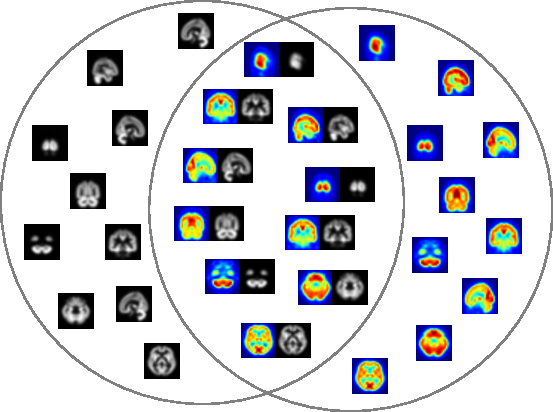
\includegraphics[width=0.8\columnwidth]{./tex/fig/nimg_scheme.pdf}
\caption{
	Pictorial example of training an imaging dataset with two views: MRI (left side, in gray scale) and FDG-PET (right side, in color scale).
	In this case we have data from 30 independent observations:
	$10$ with left-views only; $10$ with right-views only; $10$ with complete views.
	The fraction of observations with complete views amounts to: $f = 1/3$.
}
\label{fig:nimg_scheme}
\end{figure}
%
% \begin{figure*}[!t]
% \centering
% 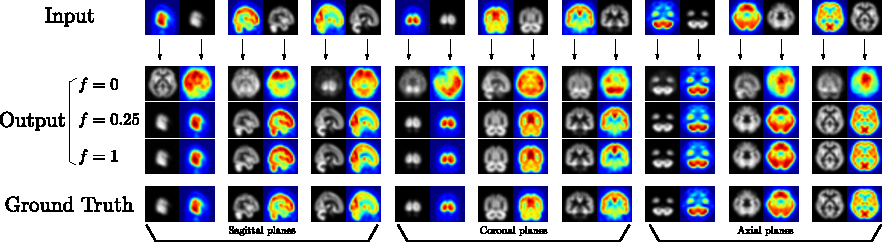
\includegraphics[width=\textwidth]{./tex/fig/nimg_test.pdf}
% \caption{
% 	Reconstruction of test-set images when MT-MCVAE models are trained with an increasing fraction ($f$) of observations with complete-views.
% 	The MRI of each subject is inferred from the FDG and \textit{vice versa}.
% 	When there are no joint observations in the training-set ($f=0$) the model cannot infer the correct joint relationship between views and generates inconsistent predictions.
% }
% \label{fig:nimg_test}
% \end{figure*}
